\section{Introduction}

Given a grammar $G$, the syntax analyzer reads a source string and: 
\begin{enumerate}
    \item If the string belongs to the language $L(G)$, then exhibits a derivation or builds a syntax tree of the string. 
    \item Otherwise, it stops and notifies the error, possibly with a diagnostic.
\end{enumerate}
If the source string is ambiguous, the result of the analysis is a set of derivations, also called forest of trees. 
There are two analyzer classes depending on whether the derivation is rightmost or leftmost, and on the reconstruction order of the derivation. 
\begin{definition}
    The \emph{bottom-up analysis} constructs the rightmost derivation in inverse order and analyzes the tree from leaves to root through reductions. 

    The \emph{top-down analysis} constructs the leftmost derivation in direct order and analyzes the tree from root to leaves through expansions. 
\end{definition}
\begin{example}
    Consider the string $aabbbaaaa$ generated by the grammar: 
    \[
    \begin{cases}
        S \rightarrow aSAB \\
        S \rightarrow b \\
        A \rightarrow bA \\
        B \rightarrow cB \\
        B \rightarrow a \\
    \end{cases}    
    \]
    The tree corresponding to the top-down analysis of the given string is as follows: 
    \begin{figure}[H]
        \centering
        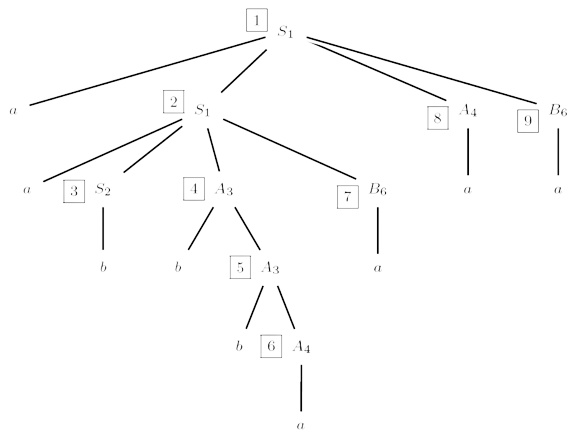
\includegraphics[width=0.5\linewidth]{images/tda.png}
    \end{figure}
    Note that the numbering indicates the application order of the rules.

    The tree corresponding to the bottom-up analysis of the given string is as follows: 
    \begin{figure}[H]
        \centering
        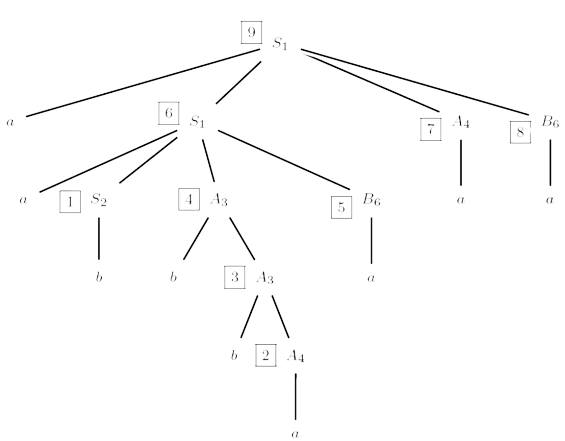
\includegraphics[width=0.5\linewidth]{images/bua.png}
    \end{figure}
\end{example}